\documentclass[11pt,a4paper]{report}
\usepackage[utf8]{inputenc}
\usepackage[T1]{fontenc}
\usepackage[spanish,es-nodecimaldot]{babel}
\usepackage{lmodern}
\usepackage[a4paper,margin=2.1cm,headheight=15pt]{geometry}
\usepackage{xcolor}
\usepackage{graphicx}
\usepackage{booktabs,tabularx,longtable,array}
\usepackage{enumitem}
\usepackage{float}
\usepackage{hyperref}
\usepackage{fancyhdr}
\usepackage[most]{tcolorbox}
\usepackage{titlesec}

\definecolor{bpnavy}{HTML}{123A55}
\definecolor{bpblue}{HTML}{1670B8}
\definecolor{bppale}{HTML}{EAF3FA}
\definecolor{bpink}{HTML}{172B3D}
\definecolor{bpmuted}{HTML}{64798C}
\definecolor{bpgreen}{HTML}{168A72}
\definecolor{bporange}{HTML}{B86E13}
\hypersetup{colorlinks=true,linkcolor=bpblue,urlcolor=bpblue,citecolor=bpnavy,pdftitle={Auditoría y preparación de despliegue | BP Digital},pdfauthor={Equipo BP Digital}}
\pagestyle{fancy}
\fancyhf{}
\lhead{\textcolor{bpmuted}{BP Digital -- Arquitectura de banca digital}}
\rhead{\textcolor{bpmuted}{Auditoría y plan de preparación}}
\cfoot{\textcolor{bpmuted}{\thepage}}
\titleformat{\chapter}{\color{bpnavy}\normalfont\LARGE\bfseries}{\thechapter}{0.7em}{}
\titleformat{\section}{\color{bpnavy}\normalfont\Large\bfseries}{\thesection}{0.6em}{}
\titleformat{\subsection}{\color{bpblue}\normalfont\large\bfseries}{\thesubsection}{0.6em}{}
\setlist[itemize]{leftmargin=1.4em,itemsep=0.25em,topsep=0.3em}
\setlist[enumerate]{leftmargin=1.7em,itemsep=0.25em,topsep=0.3em}
\renewcommand{\arraystretch}{1.25}
\setlength{\emergencystretch}{3em}
\setlength{\tabcolsep}{4pt}
\newtcolorbox{summarybox}{colback=bppale,colframe=bpblue,boxrule=0.8pt,arc=3mm,left=3mm,right=3mm,top=2mm,bottom=2mm}
\newtcolorbox{riskbox}{colback=red!4,colframe=red!55!black,boxrule=0.8pt,arc=3mm,left=3mm,right=3mm,top=2mm,bottom=2mm}
\graphicspath{{diagramas/}}

\begin{document}
\begin{titlepage}
\pagecolor{bpnavy}\color{white}
\vspace*{1.2cm}
{\Large\bfseries BP DIGITAL}\par
\vspace{2.8cm}
{\Huge\bfseries Arquitectura de banca digital}\par
\vspace{0.5cm}
{\LARGE Auditoría técnica, experiencia móvil y preparación para AWS}\par
\vspace{1.4cm}
\rule{0.8\textwidth}{1.2pt}\par
\vspace{1.0cm}
{\large Informe de solución -- Modelos C4, seguridad OAuth 2.0/MFA, onboarding facial, notificaciones y plan de costos}\par
\vfill
\begin{tabular}{@{}ll@{}}
\textcolor{white!75}{Fecha de revisión:} & 15 de noviembre de 2026 \\
\textcolor{white!75}{Estado:} & MVP local; sin despliegue de AWS \\
\textcolor{white!75}{Plataformas:} & SPA React y app móvil Expo / React Native \\
\end{tabular}
\vspace{1.2cm}
\end{titlepage}
\nopagecolor\color{bpink}
\tableofcontents
\clearpage

\chapter*{Resumen ejecutivo}
\addcontentsline{toc}{chapter}{Resumen ejecutivo}
\begin{summarybox}
El repositorio contiene una API ASP.NET Core, una SPA web React y una app móvil React Native/Expo. Las funciones bancarias del MVP usan datos SQLite locales; el proyecto no se ha desplegado en AWS y no procesa dinero real. La API fue migrada de .NET 8 a .NET 10 LTS y pasó compilación y 27 comprobaciones de integración locales. La SPA compiló y su auditoría npm no reportó vulnerabilidades de severidad alta o crítica.
\end{summarybox}

Esta revisión incorpora una pantalla móvil de alta desde Ajustes, consentimiento explícito y un contrato HTTP autenticado para crear una sesión facial. El servicio devuelve HTTP 503 con el código FACE\_VERIFICATION\_NOT\_CONFIGURED hasta que se conecte y evalúe un proveedor nativo. No se captura ni almacena una selfie. La app puede solicitar permiso del sistema y emitir una notificación local de comprobación; la entrega push remota sigue pendiente.

\begin{riskbox}
El MVP todavía no es apto para producción ni para mover fondos. MFA real, aislamiento multiusuario con tokens Cognito, validación de infraestructura, verificación facial real, push remoto, transferencia interbancaria y costos finales de AWS no se han probado. La estimación de costos se completará junto con el usuario en AWS Pricing Calculator; este informe no inventa un subtotal.
\end{riskbox}

\section*{Estado de cierre}
\begin{tabularx}{\textwidth}{@{}>{\raggedright\arraybackslash}p{4.2cm}X@{}}
\toprule
\textbf{Componente} & \textbf{Resultado} \\
\midrule
API / .NET 10 & Restauración y compilación correctas; 27 verificaciones locales aprobadas. \\
SPA React & Compilación correcta; `npm audit` informó 0 vulnerabilidades. \\
App móvil & Typecheck aprobado en una instalación temporal; faltan pruebas en dispositivo y flujo Cognito real. \\
Alta facial & Consentimiento y contrato preparados; proveedor desactivado hasta integrar SDK nativo, cotejo documental y revisión. \\
Notificaciones & Buzón API y prueba local del sistema operativo; FCM/APNs/SNS no conectados. \\
AWS y costos & Código/diagramas de preparación; sin recursos desplegados ni total aprobado de Pricing Calculator. \\
\bottomrule
\end{tabularx}

\chapter{Alcance y método}
El alcance cubre el código del MVP en `mvp/api`, `mvp/web`, `mvp/mobile`, la plantilla Cognito, Docker, CI, contratos y documentación. Se ejecutaron compilaciones, escaneo de dependencias web y pruebas de integración de API. La inspección de XSS y SQLi fue estática y mediante payloads de prueba. No se realizó pentest, revisión de configuración en una cuenta AWS ni prueba con usuarios bancarios.

Los datos de origen, cuentas y movimientos provienen de la base de desarrollo. La aceptación de una petición `202` solo representa que el MVP local guardó una solicitud; no confirma una transferencia externa.

\chapter{Arquitectura propuesta -- C4}
\section{Contexto}
El cliente de banca accede desde web o móvil a una capa HTTP autenticada. La API valida token, scope y nivel ACR, consulta la fuente Core y el sistema de detalle a través de adaptadores futuros, y delega operaciones asíncronas y notificaciones a colas y proveedores. El límite de confianza separa clientes públicos, API, proveedores de identidad, Core y servicios cloud.

\begin{figure}[H]\centering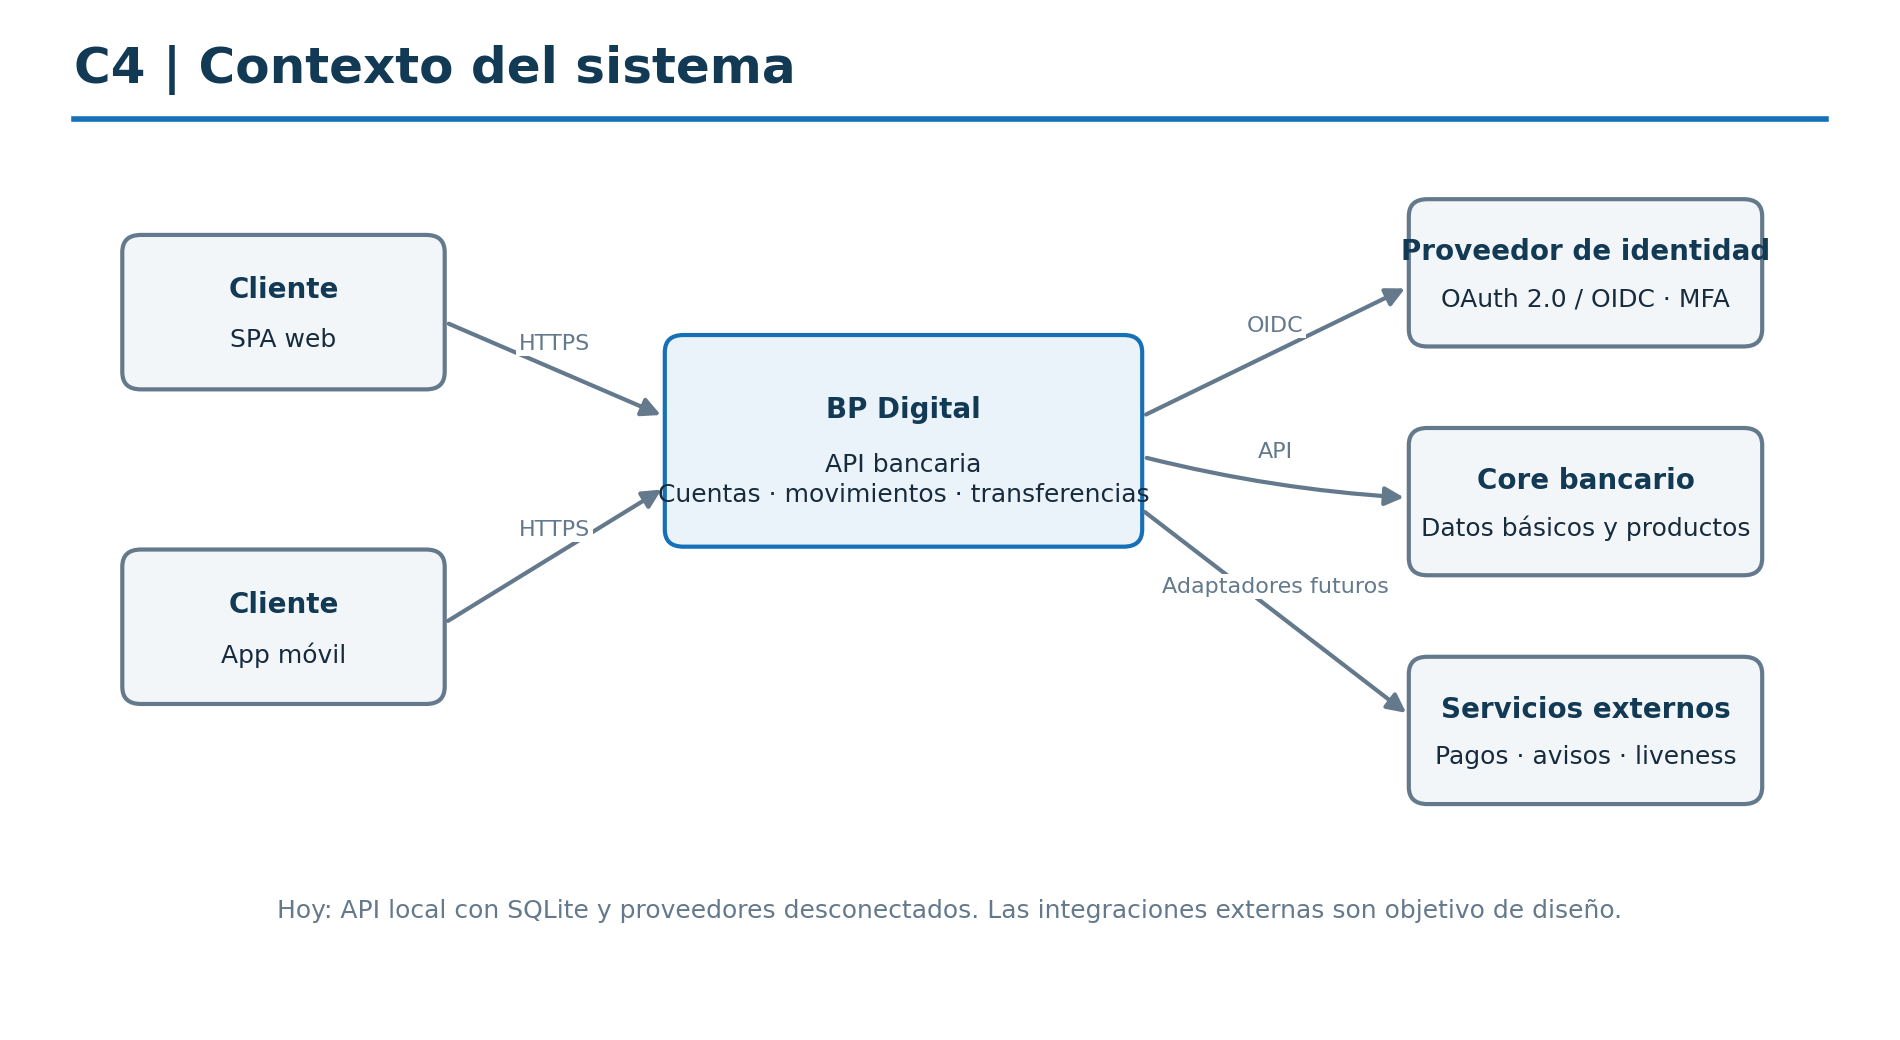
\includegraphics[width=0.98\textwidth]{c4-contexto.png}\caption{C4 -- contexto y actores externos.}\end{figure}

\section{Contenedores y componentes}
\begin{figure}[H]\centering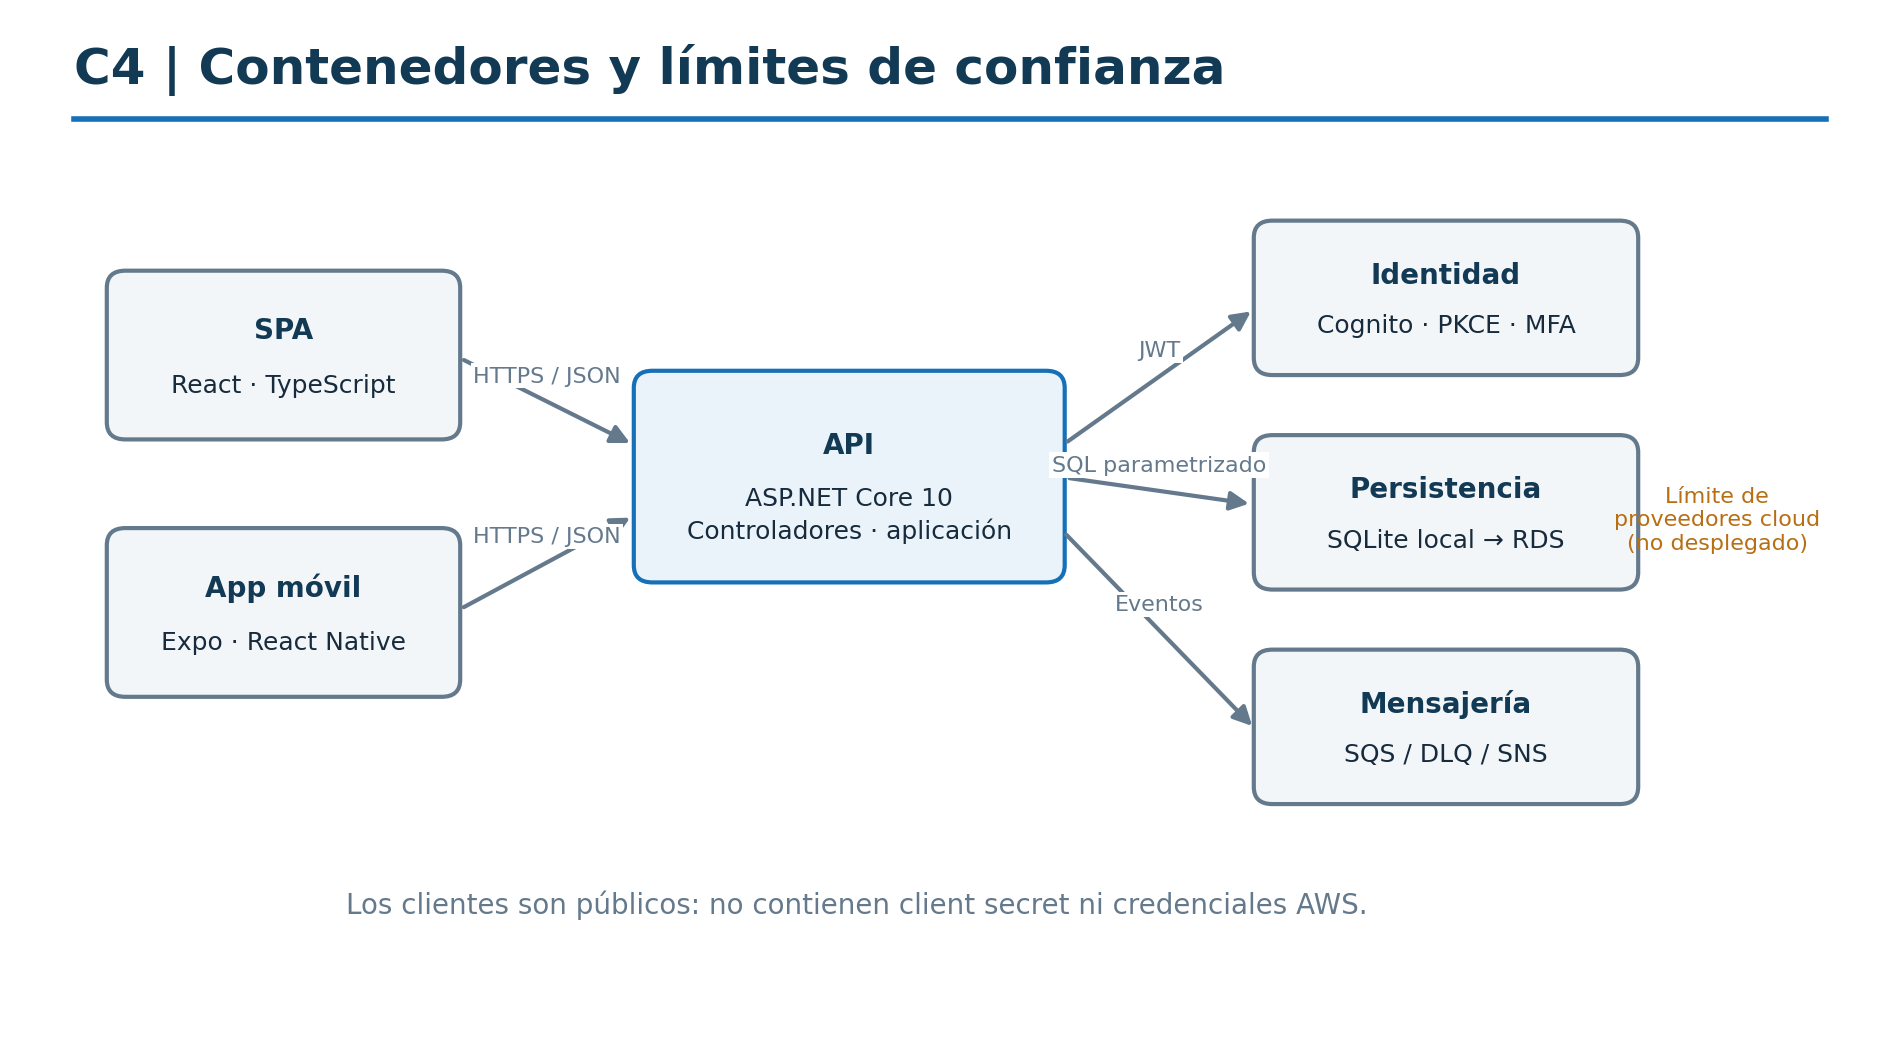
\includegraphics[width=\textwidth]{c4-contenedores.png}\caption{C4 -- contenedores previstos; los adaptadores cloud son una arquitectura objetivo, no recursos desplegados.}\end{figure}

\begin{figure}[H]\centering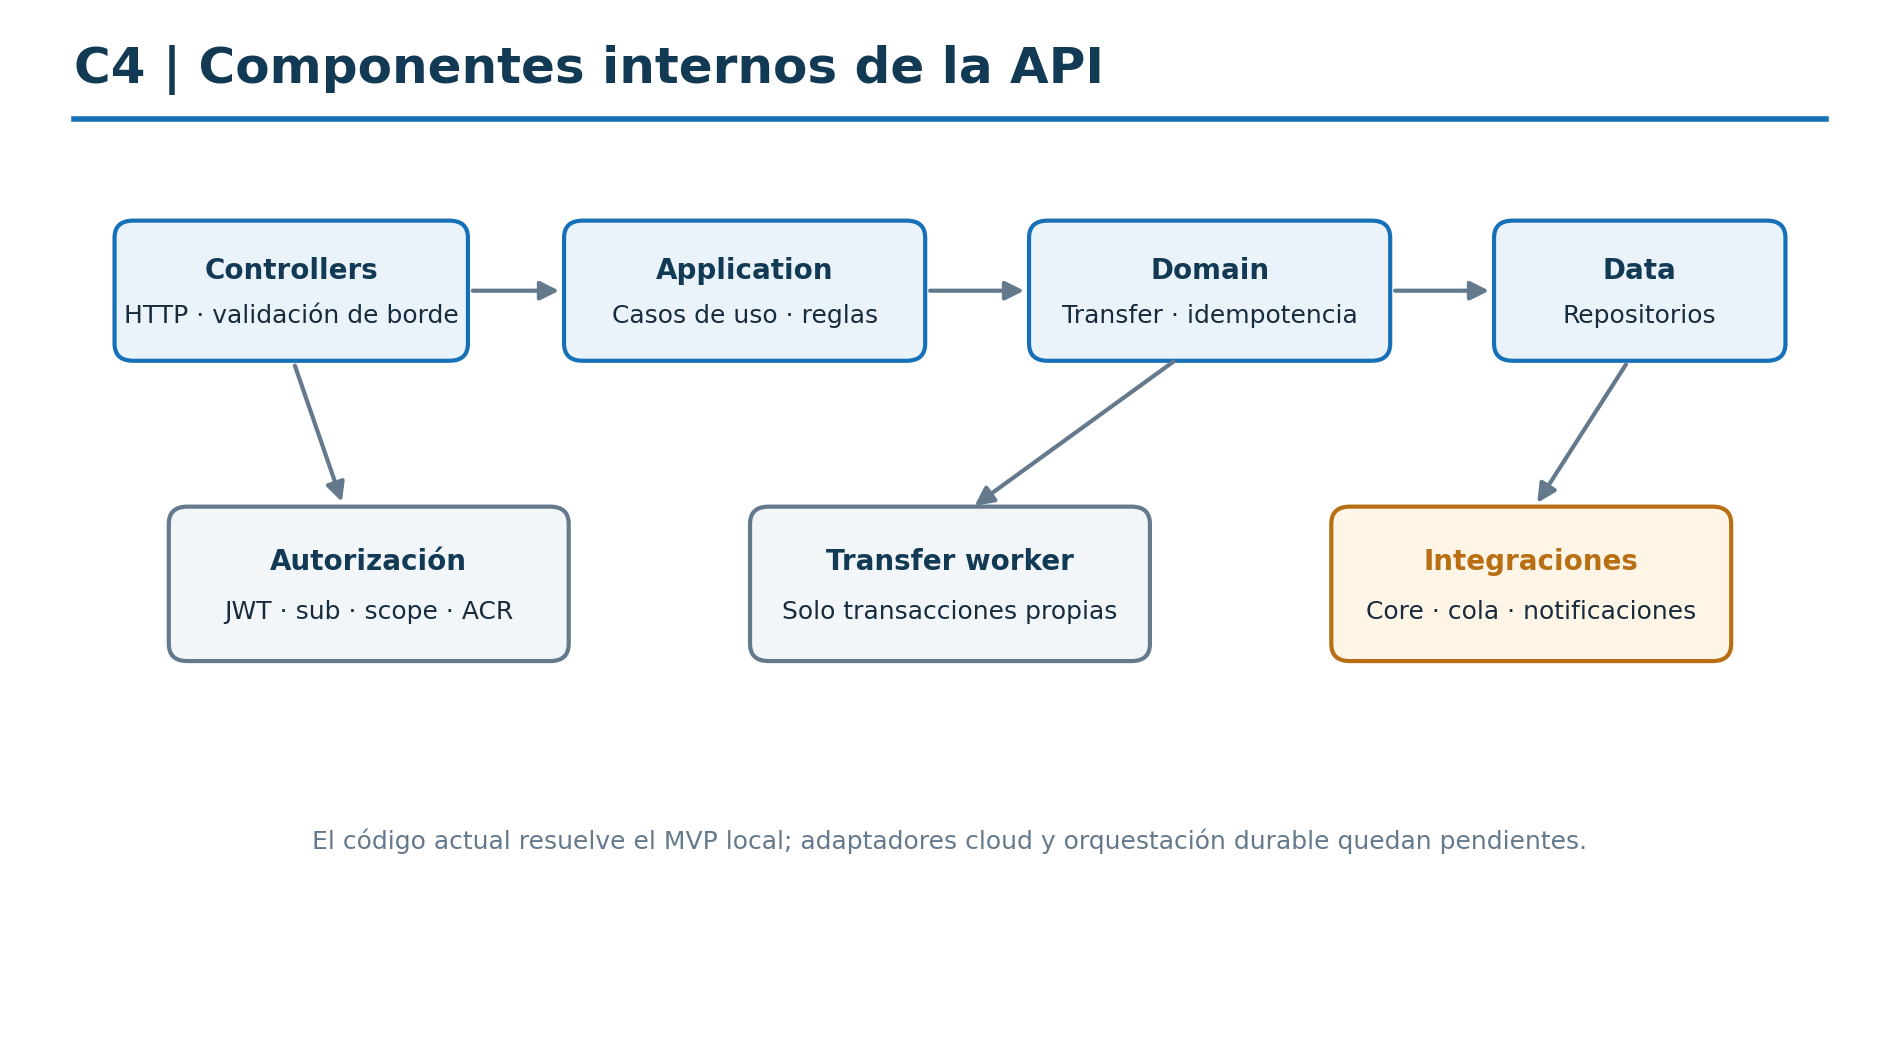
\includegraphics[width=0.96\textwidth]{c4-componentes.png}\caption{C4 -- responsabilidades internas de la API y límites de proveedor.}\end{figure}

\section{Decisiones arquitectónicas y justificación}
\begin{enumerate}
\item \textbf{Authorization Code con PKCE para SPA y móvil.} (a) Es adecuado para clientes públicos que no pueden custodiar un secreto; (b) vincula el código de autorización al iniciador de la petición y reduce su reutilización. La API valida firma/issuer, cliente, `token\_use=access`, `sub`, scope y claim `acr`.
\item \textbf{MFA centralizado en Cognito con TOTP y passkey verificada por el dispositivo.} (a) Una política del proveedor cubre ambos clientes; (b) la API puede exigir el nivel ACR alcanzado y no confiar en una bandera enviada por el cliente. La huella, rostro o PIN local protegen la clave del autenticador; son distintos de una verificación KYC.
\item \textbf{Transferencias y notificaciones desacopladas mediante outbox, cola, reintentos y DLQ.} (a) Un evento persistido evita perder una notificación si el proveedor cae; (b) idempotencia, límite de reintentos y cola de fallos dan trazabilidad y permiten recuperar mensajes sin bloquear la solicitud del cliente.
\item \textbf{RDS como fuente transaccional y DynamoDB como proyección de lectura futura.} (a) El sistema de lectura no autoriza ni debita; (b) separación de carga favorece consultas frecuentes manteniendo saldo y titularidad en las fuentes de verdad. El MVP usa SQLite local, así que la solución AWS aún requiere adaptadores y validación.
\item \textbf{Expo con desarrollo nativo para la app móvil.} (a) Comparte lenguaje y contratos TypeScript con la SPA; (b) development builds permiten módulos nativos que Expo Go no incluye. La verificación facial AWS necesita SDK nativo aprobado; no se resuelve con una alerta biométrica local.
\section{Opciones para la aplicaci\'on m\'ovil}
Se evaluaron React Native con Expo y Flutter. React Native/Expo conserva TypeScript y comparte tipos y contratos con la SPA existente; adem\'as permite usar development builds para incorporar m\'odulos nativos, por eso se mantiene en este MVP. Flutter tambi\'en es viable y ofrece widgets multiplataforma consistentes, pero introducir Dart y un segundo ecosistema aumentar\'ia la superficie de mantenimiento de este repositorio. La selecci\'on no elimina la necesidad de SDK nativo para liveness, passkeys o push remoto.

\end{enumerate}

\chapter{Auditoría de autenticación y autorización}
\section{OAuth 2.0, OIDC y MFA}
Web y móvil usan flujo Authorization Code con PKCE S256; la SPA valida `state` al volver del proveedor y guarda solo access token en `sessionStorage`. Móvil usa navegador del sistema y guarda access token/expiración en SecureStore. Ningún cliente debe incluir un client secret. Los tokens Cognito se comprueban de nuevo en la API; las rutas API requieren autorización y auditoría requiere rol `Operations`.

La plantilla de Cognito exige MFA, habilita TOTP y configuración WebAuthn con verificación del usuario, y usa Managed Login versión 2. La API acepta ACR 3 (passkey con verificación) o ACR 4 (password + TOTP). El claim ACR debe proceder del token validado y no del cuerpo HTTP. La plantilla y el callback del RP ID siguen sin probarse en una cuenta.

\begin{summarybox}
Corrección aplicada: el modo de autenticación local de la SPA solo puede activarse en build de desarrollo. El cliente móvil limpia access token ante `401` y captura errores de SecureStore durante el arranque. El refresh token/renovación aún no se implementa.
\end{summarybox}

\section{Riesgos y pruebas faltantes}
La suite local usa una identidad de desarrollo y no genera JWT firmados. Antes de habilitar usuarios hacen falta pruebas con tokens inválidos o expirados, issuer/cliente ajeno, ID token en lugar de access token, scope/ACR ausente, dos clientes distintos, rol `Operations`, revocación, step-up y recuperación de MFA. La API debe confirmar que un `sub` solo accede a su cliente y cuentas asociadas.

\chapter{Onboarding facial móvil}
El flujo objetivo informa el uso de biometría, obtiene consentimiento antes de abrir cámara, crea una sesión temporal desde API autenticada, obtiene liveness por SDK nativo, compara la referencia facial con un documento confiable y deriva resultados ambiguos a revisión humana o una alternativa accesible.

\begin{figure}[H]\centering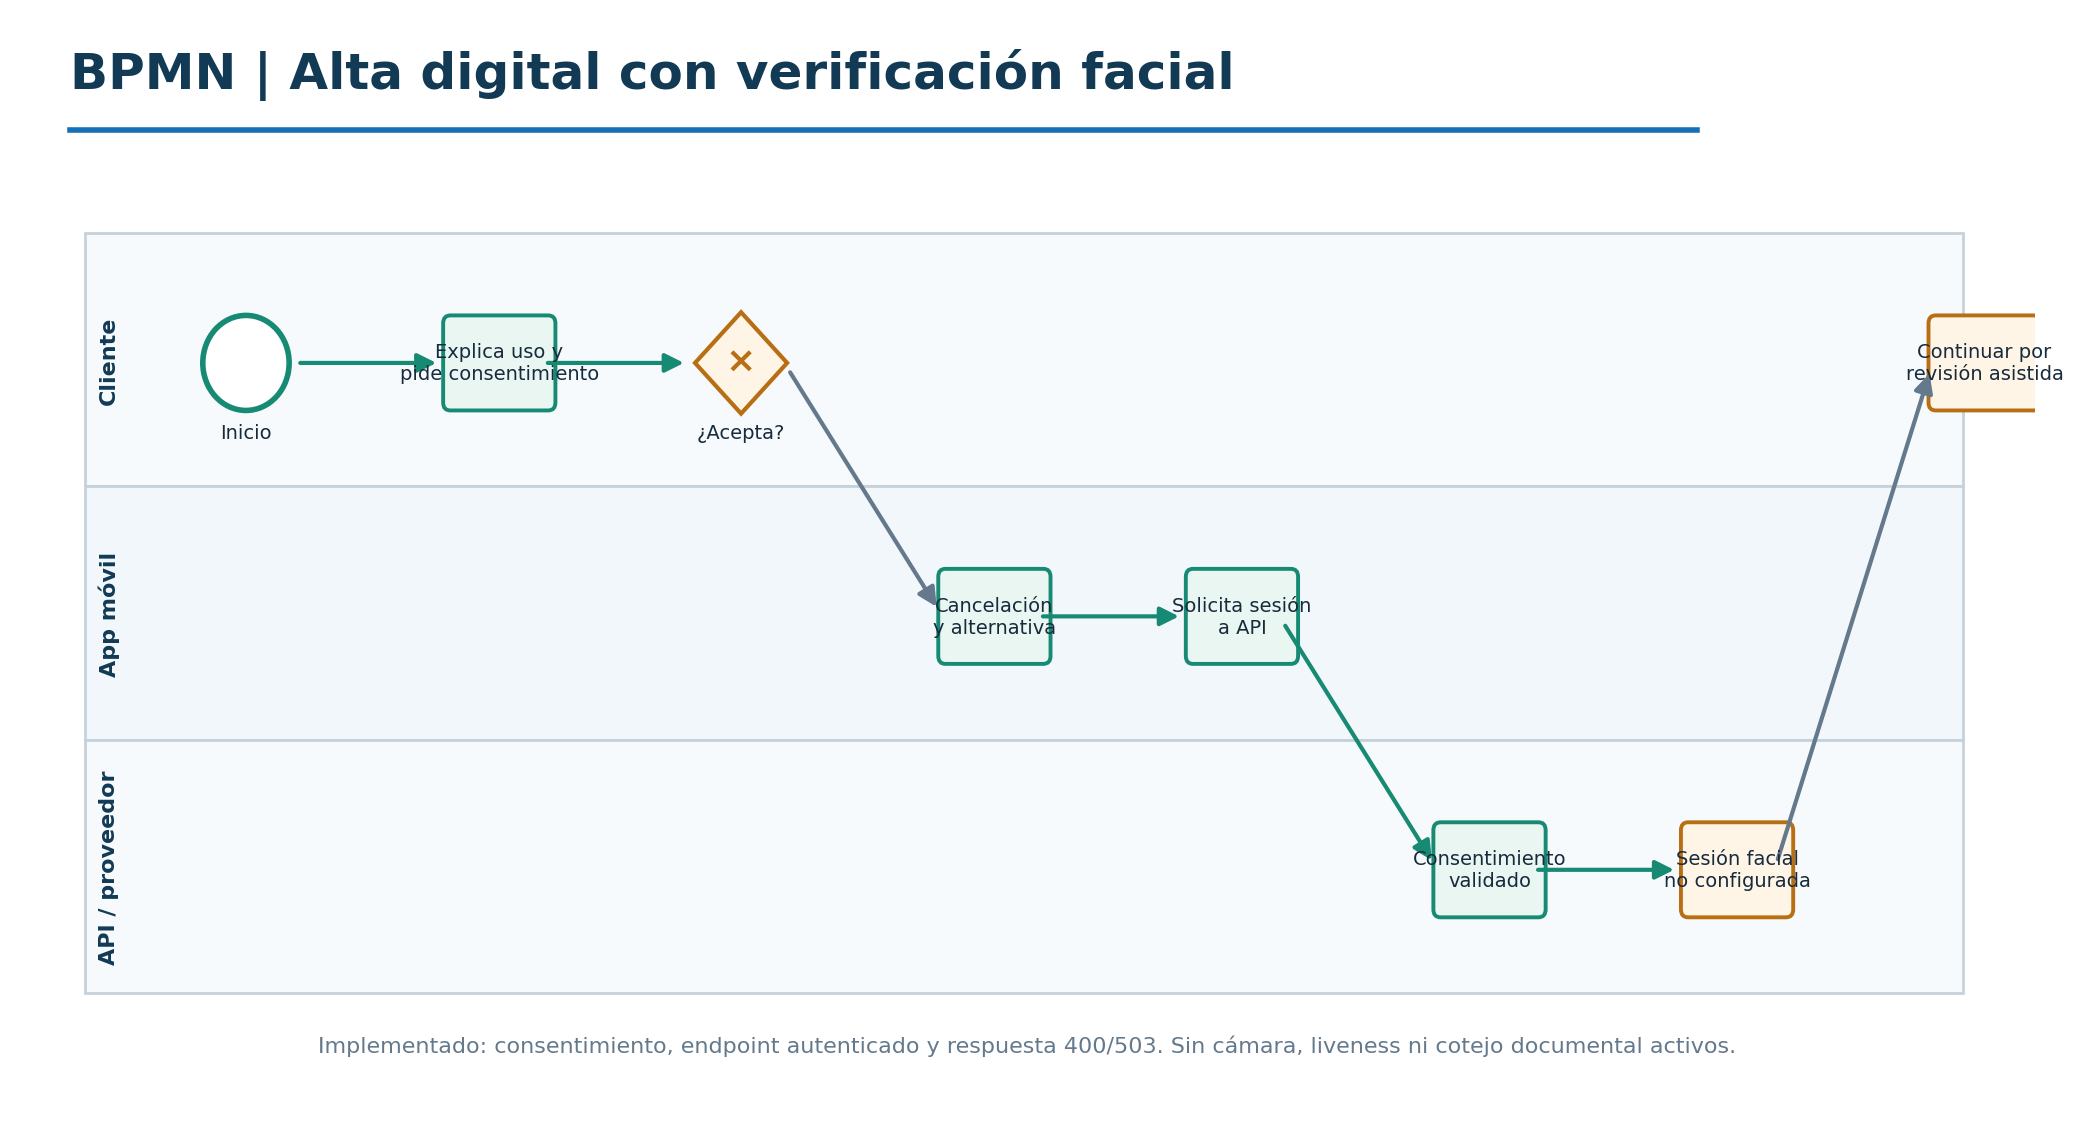
\includegraphics[width=\textwidth]{bpmn-alta-facial.png}\caption{BPMN 2.0 -- alta facial con consentimiento, comparación y revisión. El modelo editable se entrega en `diagramas/alta-facial.bpmn`.}\end{figure}

El código actual cubre el primer paso y el contrato de creación de sesión. El servidor devuelve HTTP 400 si no existe consentimiento y HTTP 503 mientras el servicio no esté configurado. La app no solicita cámara ni afirma identidad. Face Liveness verifica presencia, pero no identifica por sí sola a una persona; el cotejo requiere una imagen fuente confiable y umbrales evaluados. Deben minimizarse la retención y exposición de imagen/video, permitir ruta alternativa, explicar el tratamiento y revisar casos de alto impacto.

Para React Native con Expo se requiere seleccionar y revisar un puente nativo mantenido o implementar un módulo Expo que envuelva SDKs oficiales de iOS/Android. No se añade un paquete comunitario de bajo uso sin auditoría. El flujo no funciona en Expo Go si depende de código nativo propio; debe construirse un development client y hacer pruebas físicas en iOS y Android.

\chapter{Notificaciones del teléfono}
El centro de avisos existente lee notificaciones del API. La pantalla móvil solicita permiso del sistema, muestra su estado y programa una notificación local para validar que Android/iOS entregue un aviso. Esta prueba no demuestra push remoto.

\begin{figure}[H]\centering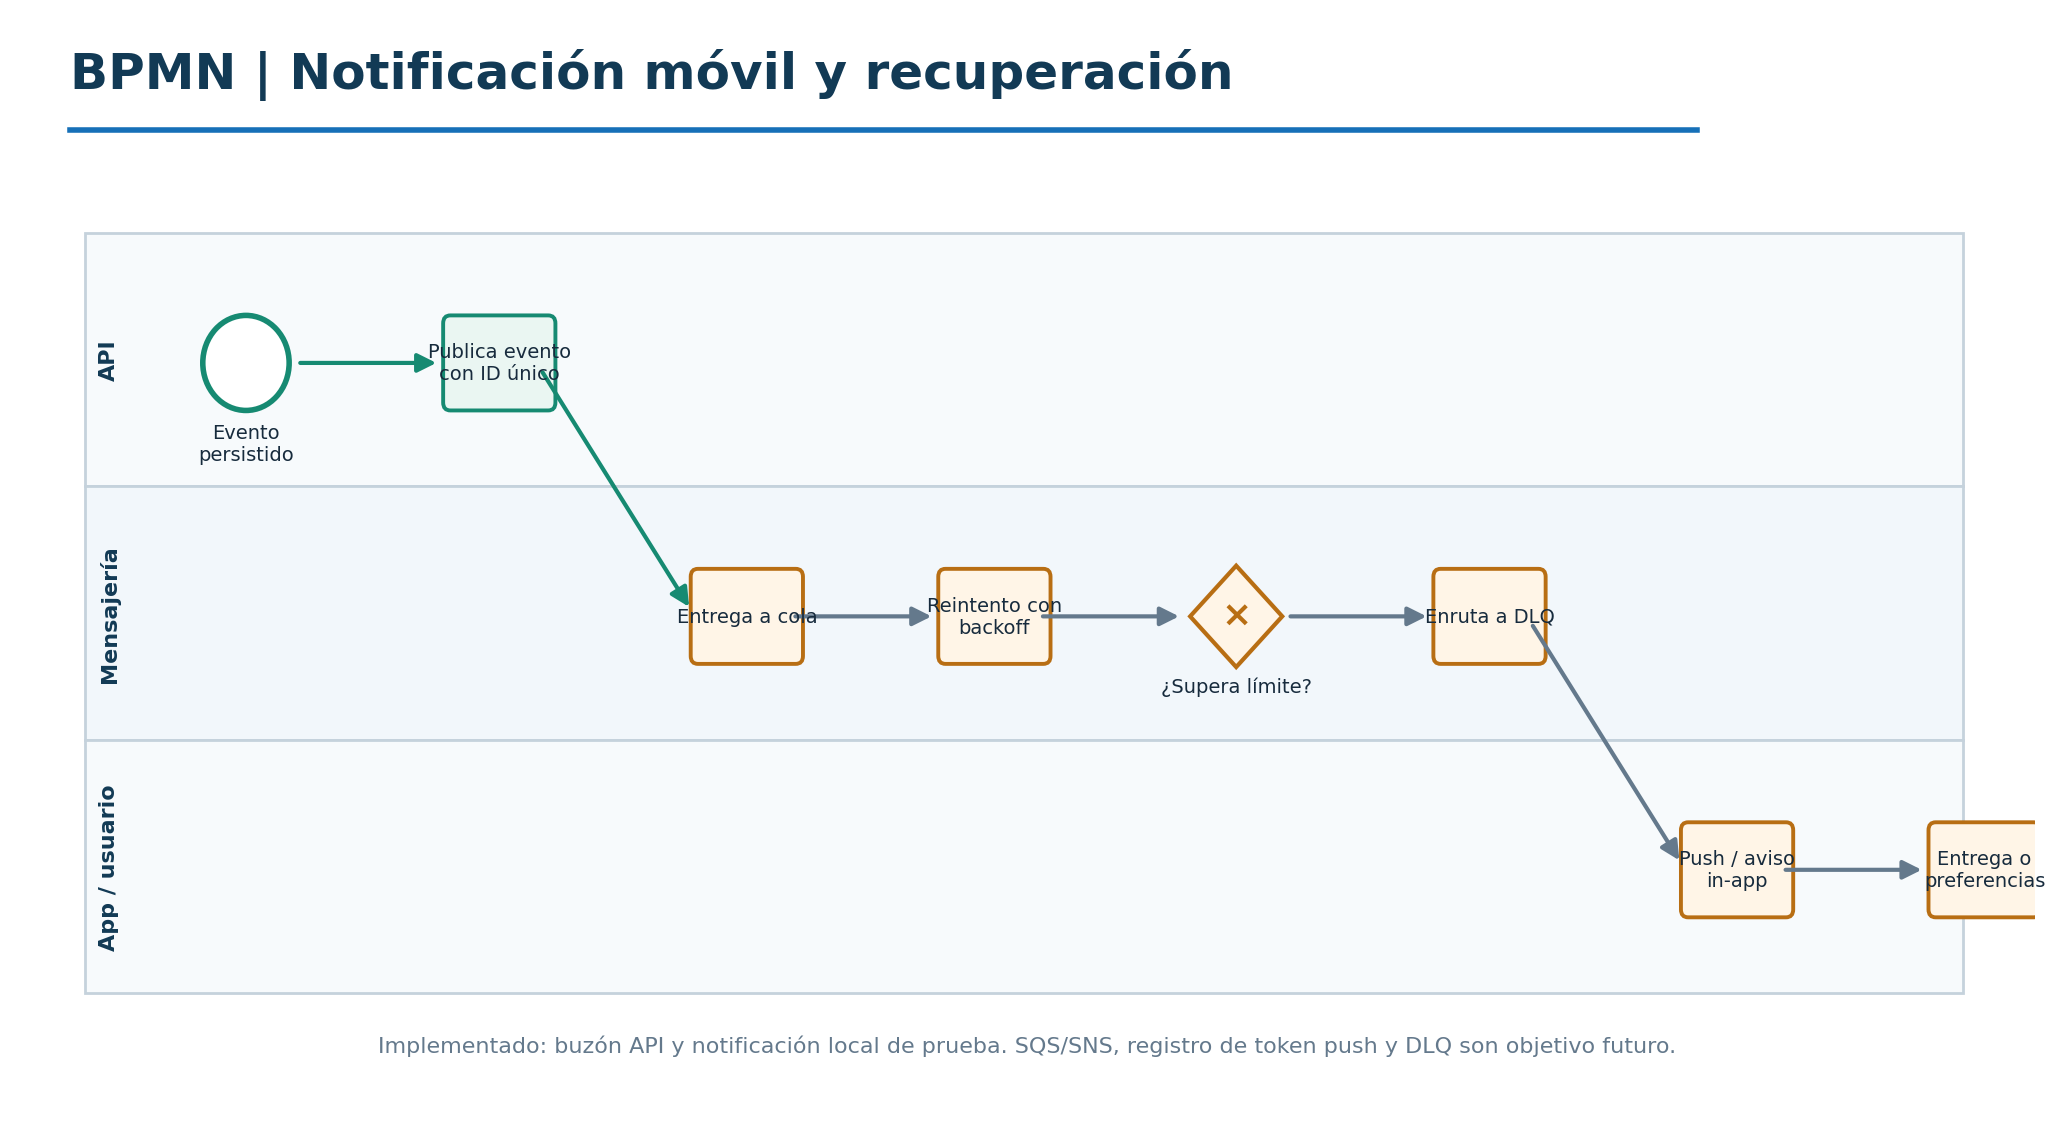
\includegraphics[width=\textwidth]{bpmn-notificaciones.png}\caption{BPMN 2.0 -- persistencia de evento, entrega multicanal y recuperación con backoff/DLQ.}\end{figure}

Para la integración futura: pedir permiso con contexto; registrar token FCM/APNs autenticado y vinculado al usuario; nunca guardar credenciales AWS en la app; publicar desde rol del backend por SNS; procesar avisos in-app y correo como consumidores independientes; limpiar tokens inválidos; incluir reintentos acotados, DLQ, métricas y preferencias del usuario. Las pruebas push exigen development build, configuración FCM/APNs y entorno AWS; la prueba local ya está implementada, pero la auditoría física queda pendiente.

\chapter{Revisión de seguridad y UX}
\section{Resultados técnicos}
\begin{itemize}
\item Las consultas de SQLite revisadas usan parámetros; los casos de entrada SQLi/XSS del test API reciben 400. No se encontró `dangerouslySetInnerHTML`/`innerHTML` en la SPA inspeccionada.
\item La auditor\'ia de paquetes NuGet no report\'o vulnerabilidades; tampoco lo hizo el an\'alisis de dependencias npm de la SPA y la app m\'ovil.
\item API devuelve Problem Details con código, traza y `X-Request-Id`; se probaron 400, 403, 404, 429, 503 y respuestas 202/200 de transferencias.
\item La transferencia usa clave idempotente y valida cuenta/monto en servidor. El worker solo completa transferencias propias; interbancarias quedan pendientes y no tienen conciliación/compensación real.
\item Docker local usa usuario no root, filesystem de solo lectura, capacidades retiradas, `no-new-privileges`, límites de recursos y bind loopback. La configuración Development/local identity no debe llevarse a producción.
\end{itemize}

\section{Matriz de ejecución}
\begin{figure}[H]\centering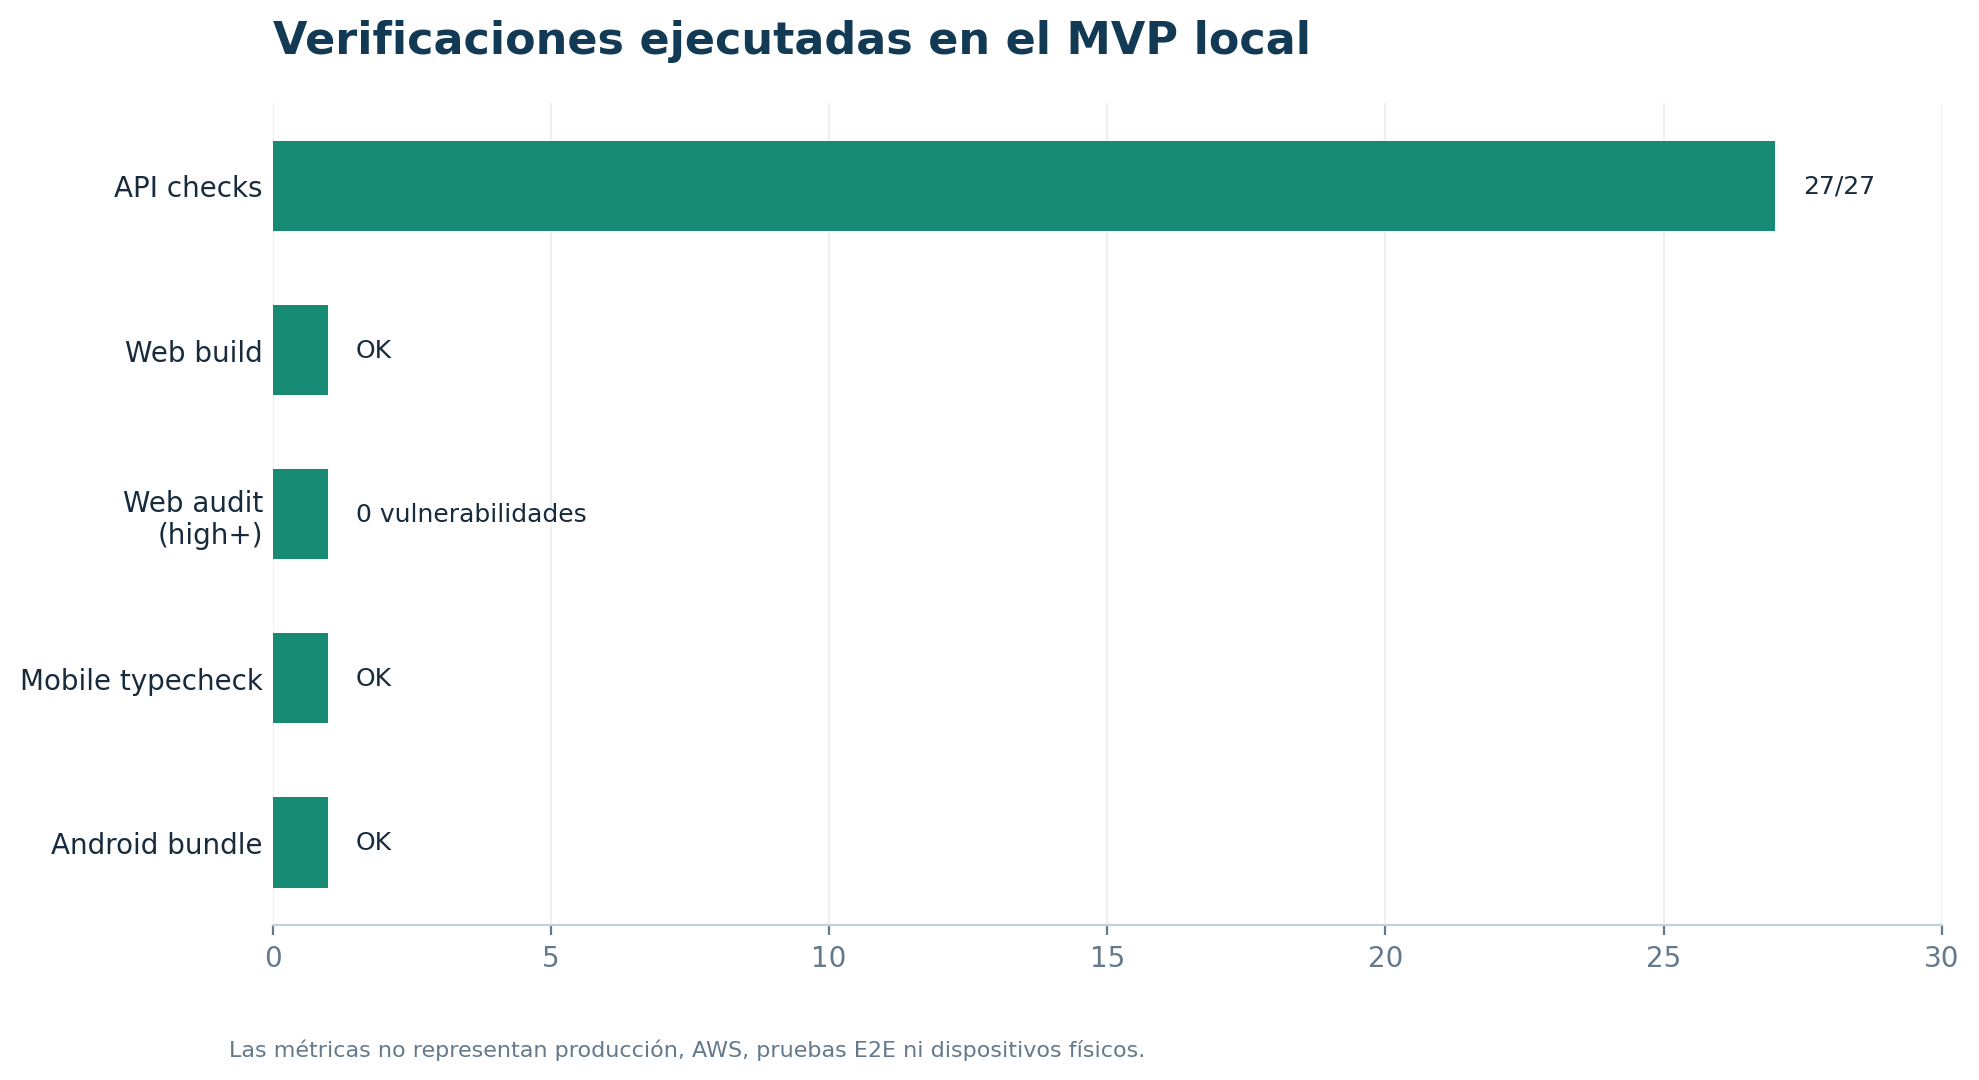
\includegraphics[width=0.83\textwidth]{resultados-pruebas.png}\caption{Resultados observados en compilación y pruebas automatizadas locales.}\end{figure}
\begin{figure}[H]\centering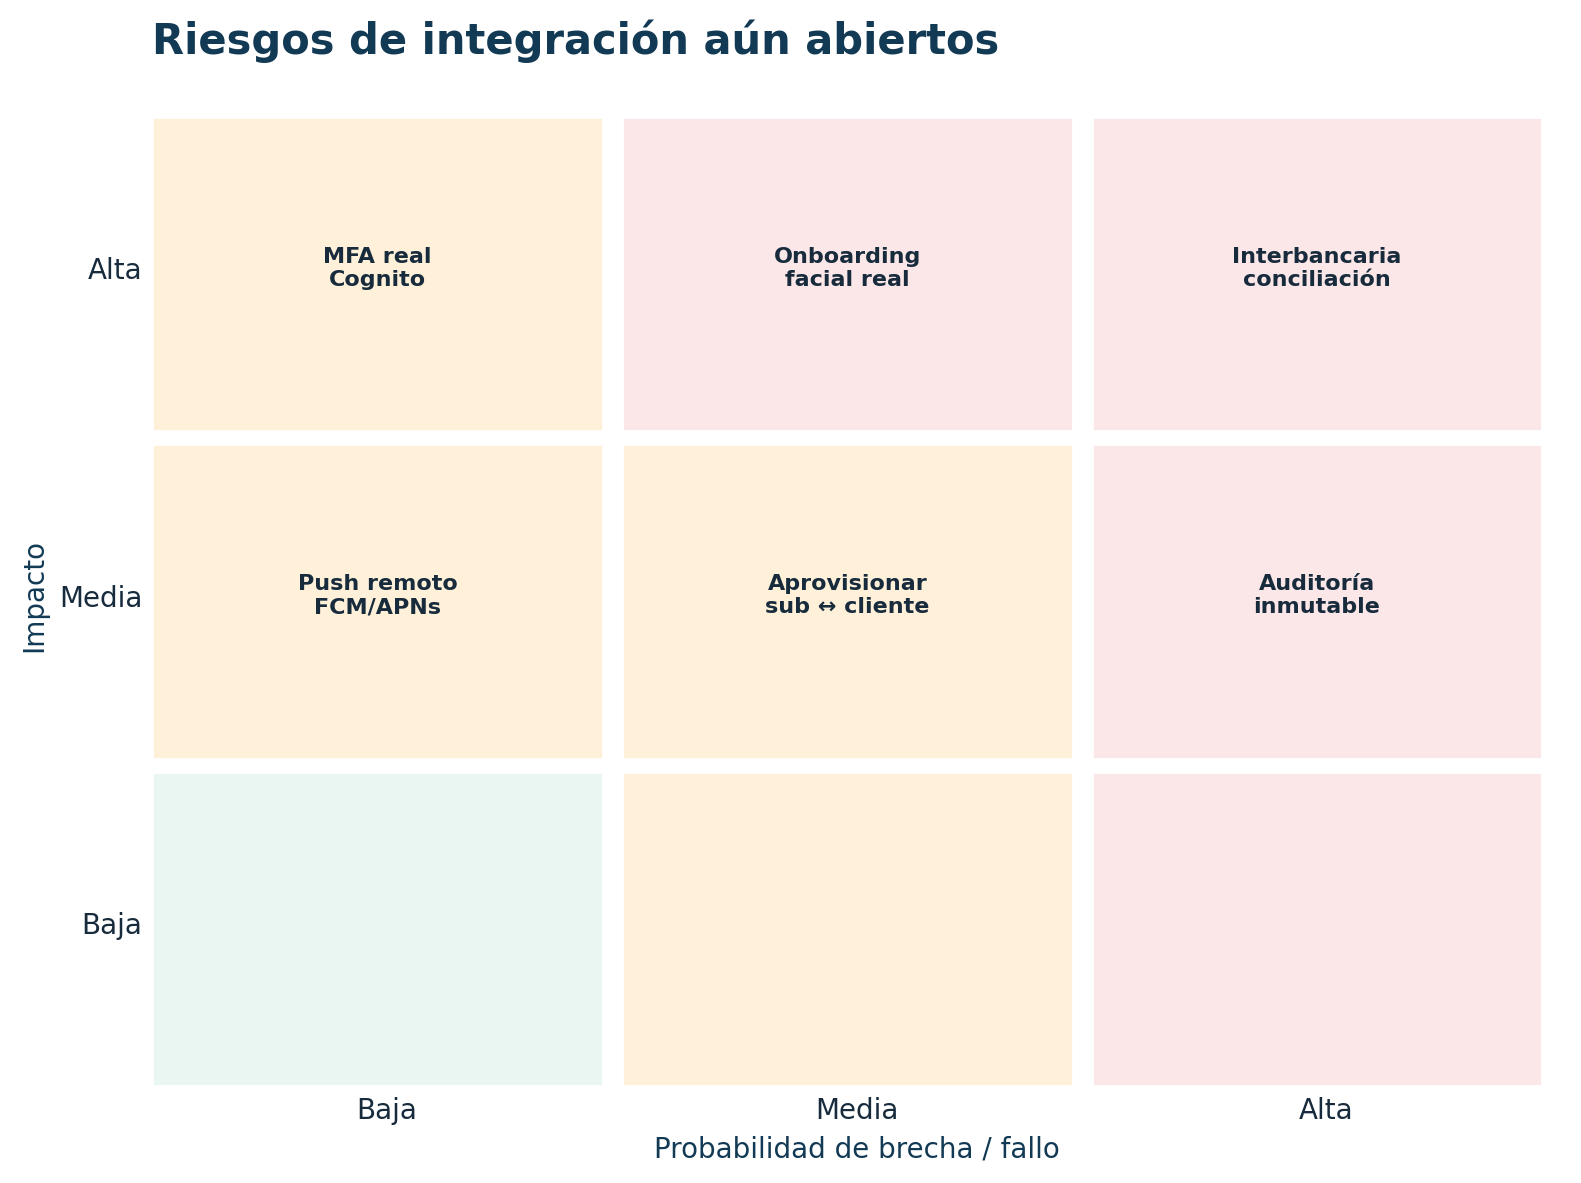
\includegraphics[width=0.7\textwidth]{matriz-riesgos.png}\caption{Riesgos abiertos de integración, priorizados cualitativamente por probabilidad e impacto.}\end{figure}

\begin{tabularx}{\textwidth}{@{}>{\raggedright\arraybackslash}p{4.2cm}X@{}}
\toprule
\textbf{Prueba} & \textbf{Resultado} \\
\midrule
API .NET 10 & `dotnet restore` y `dotnet build`: 0 warnings / 0 errors. \\
API integración & 27 comprobaciones: health, SPA, lecturas, permisos, validaciones, SQLi/XSS, idempotencia, worker, saldos, notificación, alta facial 400/503 y rate limit. \\
SPA & `npm run build`: correcto. `npm audit --audit-level=high`: 0 vulnerabilidades reportadas. \\
Móvil & `npm run typecheck`, `npm audit --audit-level=high` y `npx expo export --platform android`: correctos en una copia temporal corta con el lockfile actual. Instalación en el directorio original devolvió `EPERM`; faltan pruebas E2E, desarrollo nativo y dispositivo físico. \\
Cognito / MFA real & No probado contra AWS. \\
Push remoto / biometría facial & No probado ni conectado; los endpoints informan el estado deshabilitado. \\
\bottomrule
\end{tabularx}

\chapter{Preparación para AWS y costos}
No se creó infraestructura ni se inició despliegue. Antes de hacerlo se deben validar el template Cognito, variables y secretos en Secrets Manager/Parameter Store, roles IAM mínimos, red privada, RDS Multi-AZ, colas/DLQ, WAF, almacenamiento/retención, logging y alarmas. Se requieren pruebas de restauración, concurrencia, reintentos, expiración de tokens, entrega de push y recuperación.

\section{Normativa y marcos de control por validar}
Para operar en Ecuador, el dise\~no debe someterse a revisi\'on jur\'idica y de cumplimiento frente a la Ley Org\'anica de Protecci\'on de Datos Personales y su Reglamento General. Las im\'agenes faciales y plantillas biom\'etricas requieren evaluar finalidad, base de legitimaci\'on, transparencia, minimizaci\'on, retenci\'on, derechos y transferencias; este informe no declara cumplimiento. La Codificaci\'on vigente de la Superintendencia de Bancos incluye requisitos de seguridad de informaci\'on y ciberseguridad aplicables seg\'un el tipo de entidad y servicio. Si el alcance almacena, procesa o transmite datos de tarjetas, evaluar PCI DSS v4.0.1 y delimitar formalmente el entorno de datos de tarjeta; si no hay datos de tarjeta, no asumir que PCI DSS aplica por ser banca digital.

Como referencias de implementaci\'on, usar ISO/IEC 27001/27017/27018, NIST Cybersecurity Framework, controles OWASP para APIs y aplicaciones m\'oviles, y un proceso de respuesta a incidentes, continuidad y recuperaci\'on. El equipo legal/compliance debe determinar obligaciones regulatorias exactas, licencias, reportes al supervisor, KYC/AML, residencia y transferencia internacional de datos antes de dise\~nar el entorno de producci\'on.

\section{Modelo de costos}
La región `us-east-1` y la carga de baja demanda en `docs/aws-calculator-scenario.csv` son un escenario provisional, no confirmado por el usuario. Incluye 1.000 MAU, 10.000 solicitudes de API y 100 verificaciones faciales mensuales, además de cómputo, base de datos Multi-AZ, mensajería, almacenamiento, salida, logs, alertas e identidad. El modo DR secundario se estimará como escenario separado con RTO/RPO definidos.

No se incorpora un total en dólares porque el usuario pidió completar los valores junto con AWS Pricing Calculator y todavía faltan clase/almacenamiento RDS, CPU/memoria Fargate, transferencia saliente, retención de logs, reglas WAF, endpoints/mensajes SNS y política biométrica. El estimado compartible y el gráfico final de costos se añaden después de esa sesión. AWS Calculator ofrece estimaciones, no cotizaciones.

\begin{figure}[H]\centering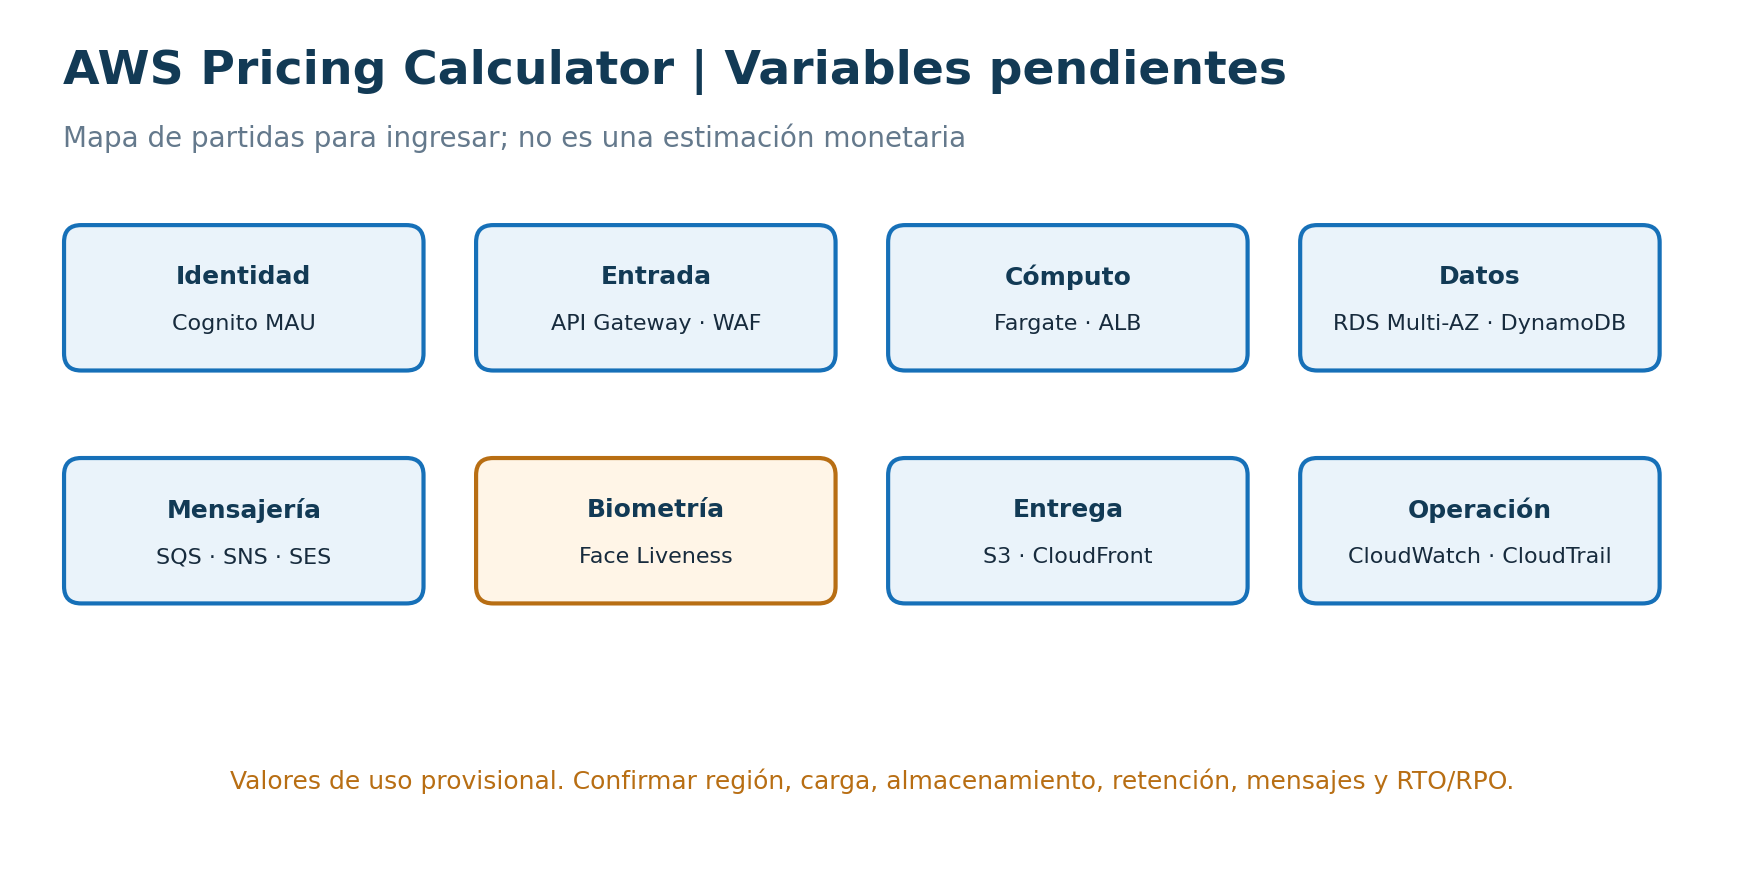
\includegraphics[width=0.92\textwidth]{modelo-costos.png}\caption{Partidas que deben introducirse en AWS Pricing Calculator; el gráfico no muestra precios ni subtotal.}\end{figure}

\chapter{Plan de cierre}
\begin{enumerate}
\item Confirmar volúmenes, región y supuestos de costo; completar y guardar enlace compartible de AWS Pricing Calculator.
\item Elegir integración facial nativa soportada y revisar privacidad, fallback, umbrales, retención y atención humana.
\item Configurar un entorno aislado Cognito; probar OAuth PKCE, MFA TOTP/passkey, claims ACR y permisos API con tokens reales.
\item Conectar notificaciones remotas con tokens móviles, SNS y segundo canal, y probar entrega/reintento/DLQ.
\item Completar acceso multiusuario, adapter Core/detalle, conciliación/compensación interbancaria, almacenamiento durable de auditoría y pruebas de caos/DR.
\item Validar CloudFormation/containers y escaneos CI; revisar el informe y luego preparar el commit/repo público con secretos y archivos locales excluidos.
\end{enumerate}

\chapter*{Referencias y herramientas}
\addcontentsline{toc}{chapter}{Referencias y herramientas}
\begin{enumerate}[label={[\arabic*]}]
\sloppy
\item Microsoft, soporte y ciclo de vida de .NET: \url{https://learn.microsoft.com/en-us/dotnet/core/releases-and-support}.
\item Amazon Cognito, niveles ACR/AMR: \url{https://docs.aws.amazon.com/cognito/latest/developerguide/cognito-user-pools-step-up-authentication.html}.
\item AWS Rekognition, Face Liveness: \url{https://docs.aws.amazon.com/rekognition/latest/dg/face-liveness.html}.
\item AWS, recomendaciones de Face Liveness, rutas alternativas y límites de intentos: \url{https://docs.aws.amazon.com/rekognition/latest/dg/recommendations-liveness.html}.
\item AWS AI Service Card, uso responsable, cotejo y revisión humana: \url{https://docs.aws.amazon.com/ai/responsible-ai/rekognition-face-liveness/overview.html}.
\item Expo, notificaciones: \url{https://docs.expo.dev/versions/latest/sdk/notifications/}.
\item Expo, notificaciones push y development builds: \url{https://docs.expo.dev/push-notifications/overview/}.
\item BPMN.io / bpmn-js, modelo BPMN 2.0, import/export y SVG: \url{https://bpmn.io/toolkit/bpmn-js/walkthrough/} y \url{https://bpmn.io/toolkit/bpmn-js/walkthrough/exporting}.
\item AWS Pricing Calculator: \url{https://calculator.aws/}. El estimador no es cotización.
\item Ecuador, Ley Org\'anica de Protecci\'on de Datos Personales, Registro Oficial, Quinto Suplemento No. 459: \url{https://www.registroficial.gob.ec/quinto-suplemento-al-registro-oficial-no-459/}.
\item Ecuador, Reglamento General de la LOPDP, Registro Oficial, Tercer Suplemento No. 435: \url{https://www.registroficial.gob.ec/tercer-suplemento-al-registro-oficial-no-435/}.
\item Superintendencia de Bancos del Ecuador, Codificaci\'on de las Normas de la SB, seguridad de la informaci\'on y ciberseguridad: \url{https://www.superbancos.gob.ec/bancos/descargas/40954/}.
\item PCI Security Standards Council, Biblioteca de documentos PCI DSS v4.0.1: \url{https://www.pcisecuritystandards.org/es/document_library/}.
\end{enumerate}

\end{document}
